% 2009-11-03
\nr
\paragraph{Theorem: }

Jedem Vektor $\vec{B}$ des reziproken gitters entspricht eine Schar
(Menge) von Kristallebenen im realen Gitter, die $\perp$ zu $\vec{B}$
ist mit Abstand 

$d=\dfrac{2\pi}{\left|\vec{B}\right|}$ 


\paragraph{Brioullin-Zone\label{par:Brioullin-Zone}}

Elementarzelle des reziproken Gitters


\subparagraph{Definiton:}

Die Wigner-Seitz-Zelle des reziproken Gitters hei\ss t 1. Brioullin-Zone\index{Brioullin-Zone}
(BZ) 

Das reziproke Gitter kann l\"uckenlos mit 1. BZ aufgef\"ullt werden

n\"achste Gitterpunkte, Mittelsenkrechte

images/2009-11-03-wigner\_seitz.gif

Weitere BZ: Mittelsemkrechten-Ebene auf Verbindungslinien weiter
entfernter Gitterpunkte


\paragraph{Theorem:}

$n$. BZ: alle BZ haben das gleiche Volumen


\paragraph{Bedeutung:}

Darstellung der Dispersionsrelation $E\left(\vec{k}\right)$ im reziproken
Raum (Phononen, Elektronen)


\paragraph{Allgemeines zur Beugung:}

Beugung an periodischen Strukturen

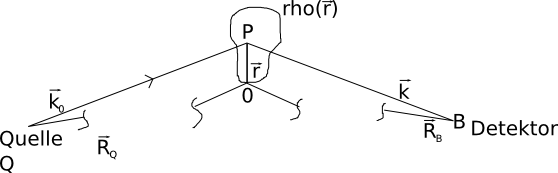
\includegraphics[scale=1]{images/2009-11-03-2-beugung.png}

Analogie zur Optik, Beugung an Gitter

$\lambda\approx\text{Gitterkonstante}$

R\"ontgenlicht, Elektronen, Neutronen


\subparagraph{Voraussetzungen:}
\begin{enumerate}
\item Einfachstreuung 
\item Fraunhofer-N\"aherung: einlaufende und gebeugte Welle werden als ebene
Wellen angen\"ahert
\item In diesem Kapitel: nur elastische Streuung
\end{enumerate}
momentane $A$ der am Ort $P$ einlaufenden Welle:

vorher $\vec{k}_{0}$

\begin{eqnarray}
A^{P} & = & A_{0}e^{i\left(\vec{k}_{0}\left(\vec{r}-\vec{R}_{Q}\right)-\omega_{0}t^{\prime}\right)}\label{eq:beugungswelle}\end{eqnarray}
 $\;(*)$ 

$\vec{R}_{Q}$ Ort der Quelle $\vec{r}$ Ort $P$ 

Amplitude und Phasenlage werden durch Streuung ver\"andert: $\rho\left(\vec{r}\right)$
komplex 

Beispiel f\"ur R\"ontgen $\rho\left(\vec{r}\right)\sim$ Elektronendichte

Amplitude am Ort $B$ des Detektors $\vec{R}_{B}$, nachher $\vec{k}$ 

$A^{B}=cA^{P}\rho\left(\vec{r}\right)\dfrac{e^{i\left[\vec{k}\left(\vec{R}_{B}-\vec{r}\right)-\omega t_{0}^{\prime\prime}\right]}}{\underbrace{\left|\vec{R}_{B}-\vec{r}\right|}_{\approx\left|\vec{R}_{B}\right|\text{ weil }\left|R_{B}\right|\gg\left|\vec{r}\right|}}$ 

$\approx\underbrace{c\dfrac{A_{0}}{\left|R_{B}\right|}e^{i\left(-\vec{k}_{0}\vec{R}_{Q}+\vec{k}\vec{R}_{B}\right)}}_{\text{konstant f\"ur feste Anordnung}}\cdot\underbrace{\rho\left(\vec{r}\right)e^{i\vec{r}\left(\vec{k}_{0}-\vec{k}\right)}}_{\text{sepz. f\"ur P }\Rightarrow\text{Summation erforderlich \"uber Probevolumen}}\cdot\underbrace{e^{i\omega_{0}\left(t^{\prime}+t^{\prime\prime}\right)}}_{\text{es wird \"uber Zeit gemittelt}}$ 

$A^{B}\sim c\intop_{\text{Volumen der Probe}}\rho\left(\vec{r}\right)e^{i\vec{r}\left(\vec{k}-\vec{k}_{0}\right)}\text{d}^{3}\vec{r}$
Fouriertransformation $\rho\mbox{\ensuremath{\left(\vec{r}\right)} }$ 

$\vec{k}-\vec{k}_{0}=\vec{K}$ Streuvektor

Phasenproblem:

i.\,A. nur $\left|A_{B}\right|^{2}=I$ Intensit\"at me\ss bar $\Rightarrow$
Phaseninformation fehlt, Umkehrung der FT nicht m\"oglich

Ausweg: 
\begin{enumerate}
\item Annahme eines bestimmten $\rho\left(\vec{r}\right)$, Berechnung von
$I$, Vergleich
\item Mehrfachstreuung ber\"ucksichtigen $\rightarrow$ dynamische Theorie 
\end{enumerate}

\paragraph{Beugung an periodischen Strukturen:}

$\vec{r}$ Vektor zum Punkt $P$ $\vec{R}$ Gittervektor $\vec{r}_{\alpha}$
zum Mittelpunkt des Atoms $\alpha$

$\vec{r}^{\prime}$ zum Punkt $P$ 

$\vec{r}=\vec{R}+\vec{r}_{\alpha}+\vec{r}^{\prime}$

$A^{B}=\intop_{V}\rho\left(\vec{r}\right)e^{-i\left(\vec{R}+\vec{r}_{\alpha}+\vec{r}^{\prime}\right)\vec{K}}\text{d}^{3}\vec{r}$

$\underbrace{\sum_{\text{alle EZ, alle}\vec{R}}e^{-i\vec{K}\vec{R}}}_{\text{Gitterfaktor}}\cdot\underbrace{\sum_{\text{alle Atome }\alpha}e^{i\vec{K}\vec{r}_{\alpha}}\cdot\underbrace{\left[\intop_{\text{Volumen Atome }\alpha}\rho_{\alpha}\left(\vec{r}^{\prime}\right)e^{-i\vec{K}\vec{r}^{\prime}}\text{d}^{3}\vec{r}^{\prime}\right]}_{f_{\alpha}\text{ Atomstreufaktor}}}_{\text{Strukturfaktor }}$


\paragraph{Theorem:}

damit Reflexe beobachtet werden k\"onnen, m\"ussen sowohl Gitter- als
Strukturfaktor $\neq0$ sein 


\paragraph{1. Gitterfaktor}

$e^{-i\vec{K}\vec{R}}$ 

$\vec{K}\cdot\vec{R}=2\pi M\; M\in\mathbb{Z}$

Beispiel:

1.\,Dim $\vec{R}=n_{1}\vec{a}_{1}$ 

$\sum_{n_{1}=0}^{M-1}e^{-i\vec{K}n_{1}\vec{a}_{1}}=\dfrac{1-e^{iM\vec{K}\vec{a}_{1}}}{1-e^{i\vec{K}\vec{a}_{1}}}$
geometrische Summe

$I\sim\left|\right|^{2}\sim\dfrac{\sin^{2}\dfrac{1}{2}M\vec{K}\vec{a}_{1}}{\sin^{2}\dfrac{1}{2}\vec{K}\vec{a}_{1}}$
ist maximal f\"ur $\vec{K}\vec{a}_{1}=2\pi h$ $h\in\mathbb{Z}$


\paragraph{Laue-Gleichung}

$\vec{a}_{1}\vec{K}=2\pi h$ 

$\vec{a}_{2}\vec{K}=2\pi k$

$\vec{a}_{3}\vec{K}=2\pi l$ 

sind genau dann erf\"ullt, wenn $\vec{K}=\vec{B}$ 


\paragraph{Ewald- Konstruktion}

elastische Beugung $\Rightarrow\left|\vec{k}_{0}\right|=\left|\vec{k}\right|=\dfrac{2\pi}{\lambda}$
\begin{enumerate}
\item $\vec{k}_{0}$ und $\vec{k}$ in Kugel eintragen
\item $\vec{K}=\vec{k}-\vec{k}_{0}$ eintragen
\item ist $\vec{K}$ ein reziproker Gittervektor, d.\,h. liegt ein Punkt
des reziproken Gitters gerade auf Oberfl\"ache der Kugel, beim Ende
von $\vec{k}$, gibt es einen Reflex
\end{enumerate}
i.\,A. kein Reflex

M\"oglichkeiten, Reflexe zu erhalten:
\begin{enumerate}
\item Variation des Radius $\lambda$ nicht fix, sonder Bereich $\lambda_{1}<\lambda<\lambda_{2}$
\item Drehung des Kristalls
\item Pulverprobe
\end{enumerate}

\paragraph{Braggsche Beugungsbedingung}

$d=\dfrac{2\pi}{\left|\vec{B}\right|}$ Netzebenenabstand

$\sin\theta=\dfrac{\dfrac{1}{2}\left|\vec{K}\right|}{\dfrac{2\pi}{\lambda}}$

images/2009-11-03-bragg\_diffraction.png

Streubedingung: 

$\vec{K}=\vec{B}$ $\left|\vec{K}\right|=\left|\vec{B}\right|$

$\left|\vec{B}\right|=\dfrac{2\pi}{d}=\left|\vec{K}\right|=\dfrac{4\pi}{\lambda}\sin\theta\Rightarrow\lambda=2d\sin\theta$ 

Annahme von Bragg dass $hkl$ teilerfremd i.\,A. $\left|\vec{B}\right|=n\left|\vec{B}'\right|$

\[
n\lambda=2d\sin\theta\]
